
% LaTeX Report Template - customizing header and footer
\documentclass[12pt,letterpaper, leqno]{article}
\usepackage[bottom=1in, top=1in, left=1in, right=1in]{geometry}
\usepackage{amsmath,rotating}
\usepackage[scanall]{psfrag}
\usepackage{setspace}
\usepackage{bm}
\usepackage{lineno}
\usepackage{caption,graphics}
\usepackage{graphicx}
\usepackage{lscape}
\usepackage{natbib}
\usepackage[nottoc]{tocbibind}
\usepackage{indentfirst}
\usepackage{longtable}
\usepackage{sectsty}
\usepackage{color}
\usepackage{fancyhdr}
\usepackage{xspace}
\usepackage{textcomp}
\usepackage{marvosym}
\usepackage{booktabs}
\bibpunct[, ]{(}{)}{;}{a}{}{,}
\renewcommand\bibname{References}
\renewcommand\figurename{Fig.}
\captionsetup{labelsep=period, singlelinecheck=false}
%\doublespace
\def\little{\fontsize{7pt}{7pt}\selectfont}
\def\Little{\fontsize{10pt}{10pt}\selectfont}
\special{papersize=8.5in,11in}

\newcommand{\diag}{\text{diag}} 
\newcommand{\super}[1]{\ensuremath{^{\text{#1}}}}
\newcommand{\sub}[1]{\ensuremath{_{\text{#1}}}}
\newcommand{\CP}{\ensuremath{\text{CP}}\xspace} 
\newcommand{\SSB}{\ensuremath{\text{SSB}}\xspace} 

\makeatletter
\def\@xfootnote[#1]{%
  \protected@xdef\@thefnmark{#1}%
  \@footnotemark\@footnotetext}
\makeatother

\begin{document}
\newcommand{\afrb}{Alaska Fishery Research Bulletin\xspace}
\newcommand{\ajms}{African Journal of Marine Science\xspace}
\newcommand{\amb}{Advances in Marine Biology\xspace}
\newcommand{\bms}{Bulletin of Marine Science\xspace}
\newcommand{\bjssf}{Bulletin of the Japanese Society of Scientific Fisheries\xspace}
\newcommand{\cb}{Conservation Biology\xspace}
\newcommand{\cjfas}{Canadian Journal of Fisheries and Aquatic Sciences\xspace}
\newcommand{\ea}{Ecological Applications\xspace}
\newcommand{\eer}{Evolutionary Ecology Research\xspace}
\newcommand{\elet}{Ecology Letters\xspace}
\newcommand{\emod}{Ecological Modelling\xspace}
\newcommand{\ebf}{Environmental Biology of Fishes\xspace}
\newcommand{\ff}{Fish and Fisheries\xspace}
\newcommand{\fo}{Fisheries Oceanography\xspace}
\newcommand{\fr}{Fisheries Research\xspace}
\newcommand{\fb}{Fishery Bulletin\xspace}
\newcommand{\ijms}{ICES Journal of Marine Science\xspace}
\newcommand{\iccat}{Collective Volume of Scientific Papers ICCAT\xspace}
\newcommand{\jae}{Journal of Animal Ecology\xspace}
\newcommand{\jai}{Journal of Applied Ichthyology\xspace}
\newcommand{\jdc}{Journal Du Conseil International Pour L'exploration De La Mer\xspace}
\newcommand{\jdcp}{Journal Du Conseil Permanent International Pour L'exploration De La Mer\xspace}
\newcommand{\jembe}{Journal of Experimental Marine Biology and Ecology\xspace}
\newcommand{\jfb}{Journal of Fish Biology\xspace}
\newcommand{\jsr}{Journal of Sea Research\xspace}
\newcommand{\jtb}{Journal of Theoretical Biology\xspace}
\newcommand{\jfrbc}{Journal of the Fisheries Research Board of Canada\xspace}
\newcommand{\jnwafs}{Journal of Northwest Atlantic Fisheries Science\xspace}
\newcommand{\mcf}{Marine and Coastal Fisheries: Dynamics, Management, and Ecosystem Science\xspace}
\newcommand{\mb}{Marine Biology\xspace}
\newcommand{\meps}{Marine Ecology Progress Series\xspace}
\newcommand{\mfr}{Marine Fisheries Review\xspace}
\newcommand{\mpb}{Marine Pollution Bulletin\xspace}
\newcommand{\najfm}{North American Journal of Fisheries Management\xspace}
\newcommand{\nzjmfr}{New Zealand Journal of Marine and Freshwater Research\xspace}
\newcommand{\pnas}{Proceedings of the National Academy of Sciences USA\xspace}
\newcommand{\rpvrciemm}{Rapports et Proc\`es-Verbaux des R\'eunions. Conseil Internationale pour l'Exploration de la Mer\xspace}
\newcommand{\rpvrcpiemm}{Rapports et Proc\`es-Verbaux des R\'eunions. Conseil Permanent Internationale pour l'Exploration de la Mer\xspace}
\newcommand{\rfbf}{Reviews in Fish Biology and Fisheries\xspace}
\newcommand{\sajms}{South African Journal of Marine Science\xspace}
\newcommand{\tafs}{Transactions of the American Fisheries Society\xspace}

\newcommand{\anzjs}{Australian \& New Zealand Journal of Statistics\xspace}
\newcommand{\as}{Applied Statistics\xspace}
\newcommand{\csda}{Computational Statistics \& Data Analysis\xspace}
\newcommand{\ees}{Environmental and Ecological Statistics\xspace}
\newcommand{\jas}{Journal of Applied Statistics\xspace}
\newcommand{\jabes}{Journal of Agricultural, Biological, and Environmental Statistics\xspace}
\newcommand{\jasa}{Journal of the American Statistical Association\xspace}
\newcommand{\jrssb}{Journal of the Royal Statistical Society. Series B\xspace}
\newcommand{\sm}{Statistics in Medicine}



\pagestyle{plain}

\begin{titlepage}\center \large

\vspace{144pt}

Do state-space assessment models perform better than traditional statistical catch-at-age models?

\vspace{144pt}

Timothy J. Miller, Anders Nielsen, Chris Legault, Ernesto Jardim, Olav Nikolai Breivik, Jonathan Deroba, Dan Hennan, Arni Magnusson, Vanessa Trijoulet, %\footnote{Northeast Fisheries Science Center, National Marine Fisheries Service, 166 Water Street, Woods Hole, MA 02543 USA} 
and ???
\end{titlepage}

\setcounter{page}{2}
%\linenumbers

\cfoot{\thepage}

\setcounter{page}{2}
\def\fourteenbold{\fontseries{b}\fontsize{14pt}{12pt}\selectfont}
\def\twelvebold{\fontseries{b}\fontsize{12pt}{12pt}\selectfont}
\def\twelveit{\fontshape{it}\fontseries{m}\fontsize{12pt}{12pt}\selectfont}
\sectionfont{\fourteenbold}
\subsectionfont{\twelvebold}
\subsectionfont{\twelvebold}
\subsubsectionfont{\twelveit}

\setcounter{footnote}{0}


\section*{Abstract}


\pagebreak

\section*{Introduction}

\begin{itemize}
\item General notions on importance of stock assessments for fisheries management
\item Evolution of stock assessments: increase in complexity, single or multifleet, state-space vs. deterministic processes
\item Numerous models used currently in fisheries management with different modelling assumptions
\item Meta-analysis on 13 stocks to investigate how the models differ in performance according to their assumptions
\item Quick description of methods: Fit 4 models to 13 stocks and compare the predictability of the models to conclude on the forecast performance
\end{itemize}

\section*{Methods}

\begin{itemize}
\item Quick presentation of models (refer mainly to papers)
\item Table summarizing difference in assumptions between models (e.g. process error assumptions, measurement error assumptions, age-structured or no, fishing mortality model, etc.)
\item Presentation of fish stocks (summary in a table and data in supplementary material?)
\end{itemize}

\subsection*{Estimation models}

We fit four assessment models to identical data sets for each stock. Two of the models are in the class of statistical catch at age models (ASAP and A4A) and two are state+space models (WHAM and SAM). ASAP is used extensively to assess US fish stocks in the northwest Atlantic ocean. SAM and A4A are used to assess stocks in Europe. WHAM is a more recently developed model that can be configured to estimate models ranging from statistical catch at age to state-space versions with options to treat various aspects as random effects. It has not been used in management but versions have been applied to stocks of yellowtail flounder \citep{milleretal16}, redfish \citep{millerhyun18}, and Atlantic cod \citep{milleretal18}.

All models treat mortality processes use the Baranov catch equations which treat survival over the annual time interval as

\subsubsection*{WHAM models}

We fitted 4 configurations of the WHAM model to each stock data set. Two configurations are close to traditional statistical catch at age models with deterministic annual transitions in the cohorts. However, annual numbers recruit to the population are treated as independent lognormal random effects. The other two configurations are full state-space models that treat the annual cohort transitions as stochastic. The difference between the two types of each class of models is how the age composition observations are treated. In models 1 and 3 we assumed multinomial distributions with a default effective sample size. For models 2 and 4 we assumed a simple logit normal distribution similar to \citet{milleretal16} except that we treated any unobserved age classes as missing. We fit these models to determine whether there were generalalities in model performance (AIC) or retrospective patterns across the stocks. The WHAM model with the lowest AIC was used for comparison with other model frameworks.

The only differences in model configuration between stocks was in configuring selectivity for the age composition observations for the abundance indices and the catch. For many of the stocks, the range of ages used to comprise the aggregate index varied among indices. This led to some difficulties in applying a default logistic function of age, so we often estimated age-specific parameters. The general approach was to initially estimate all age-specific parameters freely to see which ages exhibited peak selectivity. Then selectivity parameters at these ages were fixed at one for final model results. The initial models cannot be used for final results because typically there is confounding of fully selected catchability with other model parameters (e.g., catchability) when all selectivity parameters are free.

\subsubsection*{Parameter Estimation}

%Abundance at age in the first year ($N_{1,a}$), fully-selected fishing mortality in the first year ($F_{f,1}$), and annual deviations in log-fully-selected fishing mortality ($\delta_{f,y}$) after the first year, mean log-recruitment ($\mu$), index catchability ($q_d$), all selectivity parameters, and process error variances ($\sigma^2_{N,j}$) are fixed effects parameters $\bm{\theta}$ estimated by ML. Abundance at age ($N_{y,a}$) after the first year ($y>1$), are treated as random effects that are integrated out to obtain the marginal likelihood.

All model frameworks use some form of maximum likelihood estimation. ASAP is programmed in AD Model Builder \citep{fournieretal12} and can be configured to use various penalties to the likelihood, but no penalties were used for any applications here. Estimation for the A4A model is programmed in R \citep{R18} and is also likelihood-based. The WHAM and SAM models are programmed using the Template Model Builder (TMB) package in R \citep{kristensenetal16} and parameters are estimated by maximizing a Laplace approximation of the marginal likelihood \citep{skaugfournier06}. To use the TMB package, the joint log-likelihood is writen as a C++ program which is compiled and accessed from R. The Laplace approximation of the marginal log-likelihood is returned when called from R and we use the ``nlminb'' function in R to minimize the negative of the Laplace approximation of the marginal log-likelihood. Empirical Bayes estimates of the state variables (random effects) are provided by the mode of posterior distributions of $\textsl{\textbf{S}}$, conditioned on the fixed effects parameters.




\subsubsection*{Diagnostics}

To get independent residuals from a state-space model the so-called `one-observation-ahead' residuals are computed. The residual for the $n$'th observation is computed by using the first $n-1$ observations to predict the $n$'th. Details can be found in \citet{thygesen2017validation}.   

\section*{Results}

\section*{Discussion}

\clearpage

\bibliographystyle{cjfas2}

\bibliography{state_space_ices}

\clearpage

\section*{Appendix}

\subsection*{WHAM model description}

The definitions for probability models describing stochastic changes in abundance at age from one year to another are identical to that given in \citet{milleretal16} and \citet{millerhyun18}. Log-abundance for ages and years greater than 1 are normally distributed conditional on the vector of numbers at age from the previous
time step,

\vspace{-12pt}
\begin{equation*}
\log\left( N_{y,a}\right) | \textbf{\textsl{N}}_{y-1} \sim \text{N}\left[f_a\left(\textbf{\textsl{N}}_{y-1}\right), \sigma_{N,j}^2\right],
\end{equation*}
for $y>1$ where $\text{N}(x,y)$ indicates a normal distribution with mean $x$ and variance $y$,

\vspace{-12pt}
\begin{equation*}
 f_a\left(\textbf{\textsl{N}}_{y-1}\right) = \left\{ 
 \begin{array}{cc}
   g(N_{y-1,1}) & \text{for}\;\;a = 1,\\
   \log\left(N_{y-1,a-1}e^{-Z_{y-1,a-1}}\right) & \text{for}\;\;1<a<A,\\
   \log\left(N_{y-1,a-1}e^{-Z_{y-1,a-1}} + N_{y-1,a}e^{-Z_{y-1,a}}\right) & \text{for}\;\;a = A,
 \end{array}\right.
\end{equation*}
$Z_{y,a} = M_{y,a}+ \sum^G_{f=1} F_{f,y,a}$ is the total mortality, and $A$ indicates the terminal age class (i.e., the ``plus group''). We assume two different variance parameters ($\sigma_{N,j}$) for the abundance at age: one for the variance of annual deviations around mean log-recruitment $\mu_s$ and one for inter-annual transitions of abundance at older ages. Define $j = 1,2$ for variance parameters for recruitment and older ages, respectively. Here we do not consider spawning biomass effects on recruitment, but Beverton-Holt and Ricker assumptions are configured options in the general model. We assume recruitment is a white noise process with $g(N_{y-1,1}) = \mu$. We treat the initial numbers at age are treated as fixed effects parameters

Annual fully-selected fishing mortality rates for fleet $f$ were parameterized as (unpenalized) deviations from the previous year,

\vspace{-12pt}
\begin{equation*}
 \log\left(F_{f,y+1}\right) = \log\left(F_{f,y}\right) + \delta_{f,y}
\end{equation*}
where $y=1,\ldots,T-1$ and $\delta_{f,y}$ are the inter-annual, deviations in log-fully selected fishing mortality. 

To relate population abundance to observed relative abundance indices and corresponding age composition, we estimate a fully-selected catchability $q_{d}$ for each index $d$. and a selectivity
Then year- and age-specific fishing mortality is parameterized by multiplying age-specific selectivity and annual fishing mortality, $ F_{f,s,y,a} = s_{f,s,y,a} F_{f,y}$, where $s_{f,s,y,a}$ is selectivity at age and sex for fishing fleet $f$. Similarly, we relate population abundance to observed relative abundance indices and corresponding age composition with a fully-selected catchability $q_{d}$ for each index $d$ and an age-specific selectivity $s_{d,a}$. For both fishing fleets and relative abundance indices, we have the same age-based logistic and age-specific parameterization options for selectivity models as the ASAP moodel.

Observed log-aggregate relative abundance indices from survey $d$ are also normally distributed,

\vspace{-12pt}
\begin{equation*}
 \log\left(I_{d,y}\right) \sim \text{N}\left[\log\left(\widehat I_{d,y}\right), \sigma^2_{d,y}\right]
\end{equation*}
where observation error variances $\sigma^2_{d,y}$ are assumed known. The predicted aggregated relative abundance index is just the sum of the predicted relative abundance index at each age,

\vspace{-12pt}
\begin{equation*}
\widehat I_{d,y} = \sum^A_{a=1} \widehat I_{d,y,a}.
\end{equation*}
where
\vspace{-12pt}
\begin{equation*}
\widehat I_{d,y,a} = q_d s_{d,a} N_{y,a} e^{- Z_{y,a} \phi_d}, 
\end{equation*}
$q_d$ is the fully-selected catchability from survey $d$, $s_{d,a}$ is the selectivity from survey $d$, and $\phi_d$ is the fraction of the year elapsed when survey $d$ occurs. 

Finally, the observed log-aggregate catches by fishing fleet $f$ are also normally distributed,

\vspace{-12pt}
\begin{equation*}
\log\left(C_{f,y}\right) \sim \text{N}\left[\log\left(\widehat C_{f,y}\right), \tau^2_{f,y}\right]
\end{equation*}
where observation error variances $\tau^2_{f,y}$ are assumed to be known. The predicted catch at age given abundances at age is
\begin{equation}\label{pred.caa}
\widehat C_{f,y,a} = \frac{F_{f,y,a}}{Z_{y,a}}\left(1 - e^{-Z_{y,a}}\right) N_{y,a} W_{f,y,a}
\end{equation}
where $W_{f,y,a}$ is the weight at age in the catch by fleet $f$. The predicted aggregated annual catch is just the sum over ages
\begin{equation}\label{pred.catch}
\widehat C_{f,y} = \sum^A_{a=1} \widehat C_{f,y,a}.
\end{equation}

We assumed a multinomial distribution for the vector of frequencies at age in survey $d$ in year $y$, 

\vspace{-12pt}
\begin{equation}\label{multinom.dist}
\textbf{\textsl{n}}_{d,y} = E_{d,y} \textsl{\textbf{p}}_{d,y} \sim \text{Multinomial}\left(E_{d,y}, \widehat {\textsl{\textbf{p}}} _{d,y}\right)
\end{equation}
where $E_{d,y}$ represented the sample size and the age-specific elements of the vector $\widehat {\textsl{\textbf{p}}} _{d,y}$ are
\vspace{-12pt}
\begin{equation*}
  \widehat p_{d,y,a} = \frac{\widehat I_{d,y,a}}{\widehat I_{d,y}}.
\end{equation*}

Similarly, we assume a multinomial distribution with sample size $E_{f,y}$ for the proportions at age in the catch,

\vspace{-12pt}
\begin{equation*}
  \widehat p_{f,y,a} = \frac{\widetilde C_{f,y,a}}{\widetilde C_{f,y}},
\end{equation*}
where $\widetilde C_{f,y,a}$ is the predicted number at age (i.e., Eq. \ref{pred.caa} with $W_{f,y,a} = 1$) and $\widetilde C_{f,y}$ is analogous to Eq. \ref{pred.catch}. However, there are options for other distributions for the age composition observations.

\subsection*{The SAM state-space assessment model}

The basic state-space assessment model (SAM) is described in \citet{nielsen2014estimation}. The model has been continuously developed and adapted for different stocks (e.g.~to include tagging data and biomass indices). The current implementation, which is available at: https://github.com/fishfollower/SAM, is an R-package based on Template Model Builder (TMB) \citep{kristensenetal16}.

The model is a state--space model. The states $\alpha$ are the log-transformed stock sizes $\log{N_1},\ldots,\log{N_A}$ and fishing mortalities $\log{F_1},\ldots,\log{F_{A}}$ corresponding to total age specific catches. It is often assumed that some age classes have the same fishing mortality. In any given year $y$ the state is the combined vector $\alpha_y$ $=$ $(\log{N_1},\ldots,\log{N_A},$ $ \log{F_1},\ldots,\log{F_{A}})'$. The transition equation describes the distribution of the next years state from a given state in the current year. The following is assumed: 
 \begin{align*}
 \alpha_{y}=T(\alpha_{y-1})+\eta_y
 \end{align*}  
 The transition function $T$ is where the stock equation and assumptions about stock--recruitment enters the model. The equations are:   
 \begin{align*}
 \log N_{1,y}&=SR(\log(N_{,y-1}))&\\
 \log N_{a,y}&=\log N_{a-1,y-1} - F_{a-1,y-1} - M_{a-1,y-1}\ , \quad &2\leq a < A \\
 \log N_{A,y}&=\log( N_{A-1,y-1}\exp^{- F_{A-1,y-1} - M_{A-1},y-1} + N_{A,y-1}\exp^{- F_{A,y-1} - M_{A,y-1}})&\\
 \log F_{a,y}&=\log F_{a,y-1}\ , \quad &1\leq a \leq A 
 \end{align*}  
Here $M_{a,y}$ is the age and year specific natural mortality parameter, which is assumed known from outside sources. $F_{a,y}$ is the total fishing mortality. The function `$SR$' is the stock-recruitment relationship assumed (options are: plain random walk on logaritmic scale, Ricker, and Beverton-Holt). 

The process noise $\eta$ is assumed to be Gaussian with zero mean, and separate variance parameters. Typically one for recruitment ($\sigma^2_{N_{a=1}}$), one for survival ($\sigma^2_{N_{a>1}}$), one for fishing mortality at age ($\sigma^2_{F}$), but these can be flexibily configured. The $N$-part of $\eta$ is assumed uncorrelated, and the $F$-part can be assumed correlated according to an AR(1) correlation structure, such that $\mbox{cor}(\Delta\log(F_{a,y}),\Delta\log(F_{\tilde{a},y}))=\rho^{|a-\tilde{a}|}$. 

The observation part of the state--space model describes the distribution of the observations for a given state $\alpha_y$. Here the vector of all observations from a given year $y$ is denoted $x_y$. The elements of $x_y$ are age-specific log-catches $\log C_{a,y}$ and age-specific log-indices from scientific surveys $\log I^{(s)}_{a,y}$.  The combined observation equation is:
 \begin{align*}
 x_y=O(\alpha_y)+\varepsilon_y
 \end{align*}
 The observation function $O$ consists of the catch equations for total catches and scientific surveys. The measurement noise term $\varepsilon_y$ is assumed to be Gaussian. An expanded view of the observation equation becomes:
 \begin{align*}
 \log C_{a,y} &= 
\log\left(\frac{F_{a,y}}{Z_{a,y}}(1-e^{-Z_{a,y}})N_{a,y}\right)+\varepsilon^{(c)}_{a,y}\\
 \log I^{(s)}_{a,y} &= 
 \log\left(Q^{(s)}_a e^{-Z_{a,y}\frac{D^{(s)}}{365}}N_{a,y}\right)+\varepsilon^{(s)}_{a,y}
\end{align*}   
Here $Z$ is the total mortality rate $Z_{a,y}=M_{a,y}+F_{a,y}$, $D^{(s)}$ is the number of days into the year where the survey $s$ is conducted, $Q^{(s)}_a$ are model parameters describing catchability coefficients. The variance of $\varepsilon_y$ is setup such that each data source catches, and the four scientific surveys have their own covariance matrix. 

Observation uncertainty is important e.g.~to get the relative weighting of the different information sources correct, so a lot of effort has been invested in getting the optimal options into SAM. In \citet{berg2016accounting} different covariance structures are compared for four ICES stocks. It was found that irregular lattice AR(1) observation correlation structure was optimal for surveys. The covariance structures tested were inspired by a previous study \citep{berg2014evaluation} of the structures obtained from survey calculations. In the paper \citet{albertsen2016choosing} 13 different observational likelihood formulations were evaluated for four ICES stocks. It was found that the multivariate log-normal representation was among the optimal in all four cases.

To describe the options available consider a yearly vector $C_y=(C_{a=1,y},\ldots,C_{a=A,y})$ of age specific observations from a fleet (survey or commercial). Assume first that the $\log(C_y)$ is multivariate Gaussian: 
\[
\log(C_y) \sim N(\log(\widehat{C}_y), \Sigma)
\]   
where $\Sigma$ is the covariance matrix, and $\hat{C}_y$ is the vector of the usual model predictions. The covariance matrix is specified from a vector of standard deviations $\sigma=(\sigma_1\ldots\sigma_A)$ and a correlation matrix $\rho$ (by $\Sigma_{a\tilde{a}}=\sigma_a\sigma_{\tilde{a}}\rho_{a\tilde{a}}$). Four options are available for the correlation $\rho$: Independent ($\rho=I$), auto-regressive of order 1 ($\rho_{a\tilde{a}}=0.5^{\theta|a-\tilde{a}|}, \ \theta>0$)\footnote[$\star$]{This parametrization is equvivalent to the more common $\phi^{|a-\tilde{a}|}$, where $0<\phi<1$}, irregular auto-regressive of order 1 ($\rho_{a\tilde{a}}=0.5^{|\theta_a-\theta_{\tilde{a}}|}, \ \theta_1=0\leq\theta_2\leq\cdots\leq\theta_A$), and unstructured (parameterized by the Cholesky of $\rho$). The options for covariance structure can be set for each fleet individually. In addition it is also possible to supply external weights for each individual observation. This option can be used in two ways. To set the relative weighting, or to actually set the fixed variance of each individual observation.

\subsubsection*{Likelihood and approximation}

The likelihood function for this is set up by first defining the joint likelihood of both random effects (here collected in the $\alpha_y$ states), and the observations (here collected in the $x_y$ vectors). The joint likelihood is:
 \begin{align*}
 L(\theta,\alpha,x)=\prod_{y=2}^Y\{ \phi(\alpha_y-T(\alpha_{y-1}),\Sigma_\eta)\}
                    \prod_{y=1}^Y\{ \phi(x_y-O(\alpha_{y}),\Sigma_\varepsilon)\}
 \end{align*}
 Here $\theta$ is a vector of model parameters. Since the random effects $\alpha$ are not observed inference should be obtain from the marginal likelihood:
 \begin{align*}
 L_M(\theta,x)=\int L(\theta,\alpha,x) d\alpha
 \end{align*}
 This integral is difficult to calculate directly, so the Laplace  approximation is used. The Laplace approximation is derived by first  approximating the joint log likelihood $\ell(\theta,\alpha,x)$ by a  second order Taylor approximation around the optimum $\hat{\alpha}$  w.r.t.~$\alpha$. The resulting approximated joint log likelihood can  then be integrated by recognizing it as a constant term and a term  where the integral is know as the normalizing constant from a  multivariate Gaussian. The approximation becomes:
 \begin{align*}
 \int L(\theta,\alpha,x)d\alpha \approx  \sqrt{\frac{(2\pi)^{n}}{\det(-\ell_{\alpha\alpha}''(\theta,\alpha,x)|_{\alpha=\hat{\alpha}_\theta})}}\exp(\ell(\theta,\hat{\alpha}_\theta,x))
 \end{align*}
 Taking the logarithm gives the Laplace approximation of the marginal log likelihood  
 \begin{align*}
 \ell_M(\theta,x) = \ell(\theta,\hat{u}_\theta,x)-\frac{1}{2}\log(\det(-\ell_{uu}
 ''(\theta,u,x)|_{u=\hat{u}_\theta}))+\frac{n}{2}\log(2\pi)
 \end{align*}

%Figures
\begin{landscape}
\begin{figure}
\caption{Degree of retrospective pattern in average fishing mortality, recruitment, and spawning stock biomass as measured by Mohn's $\rho$ for each stock and model type.}\label{rho_paper_plot}
\begin{center}
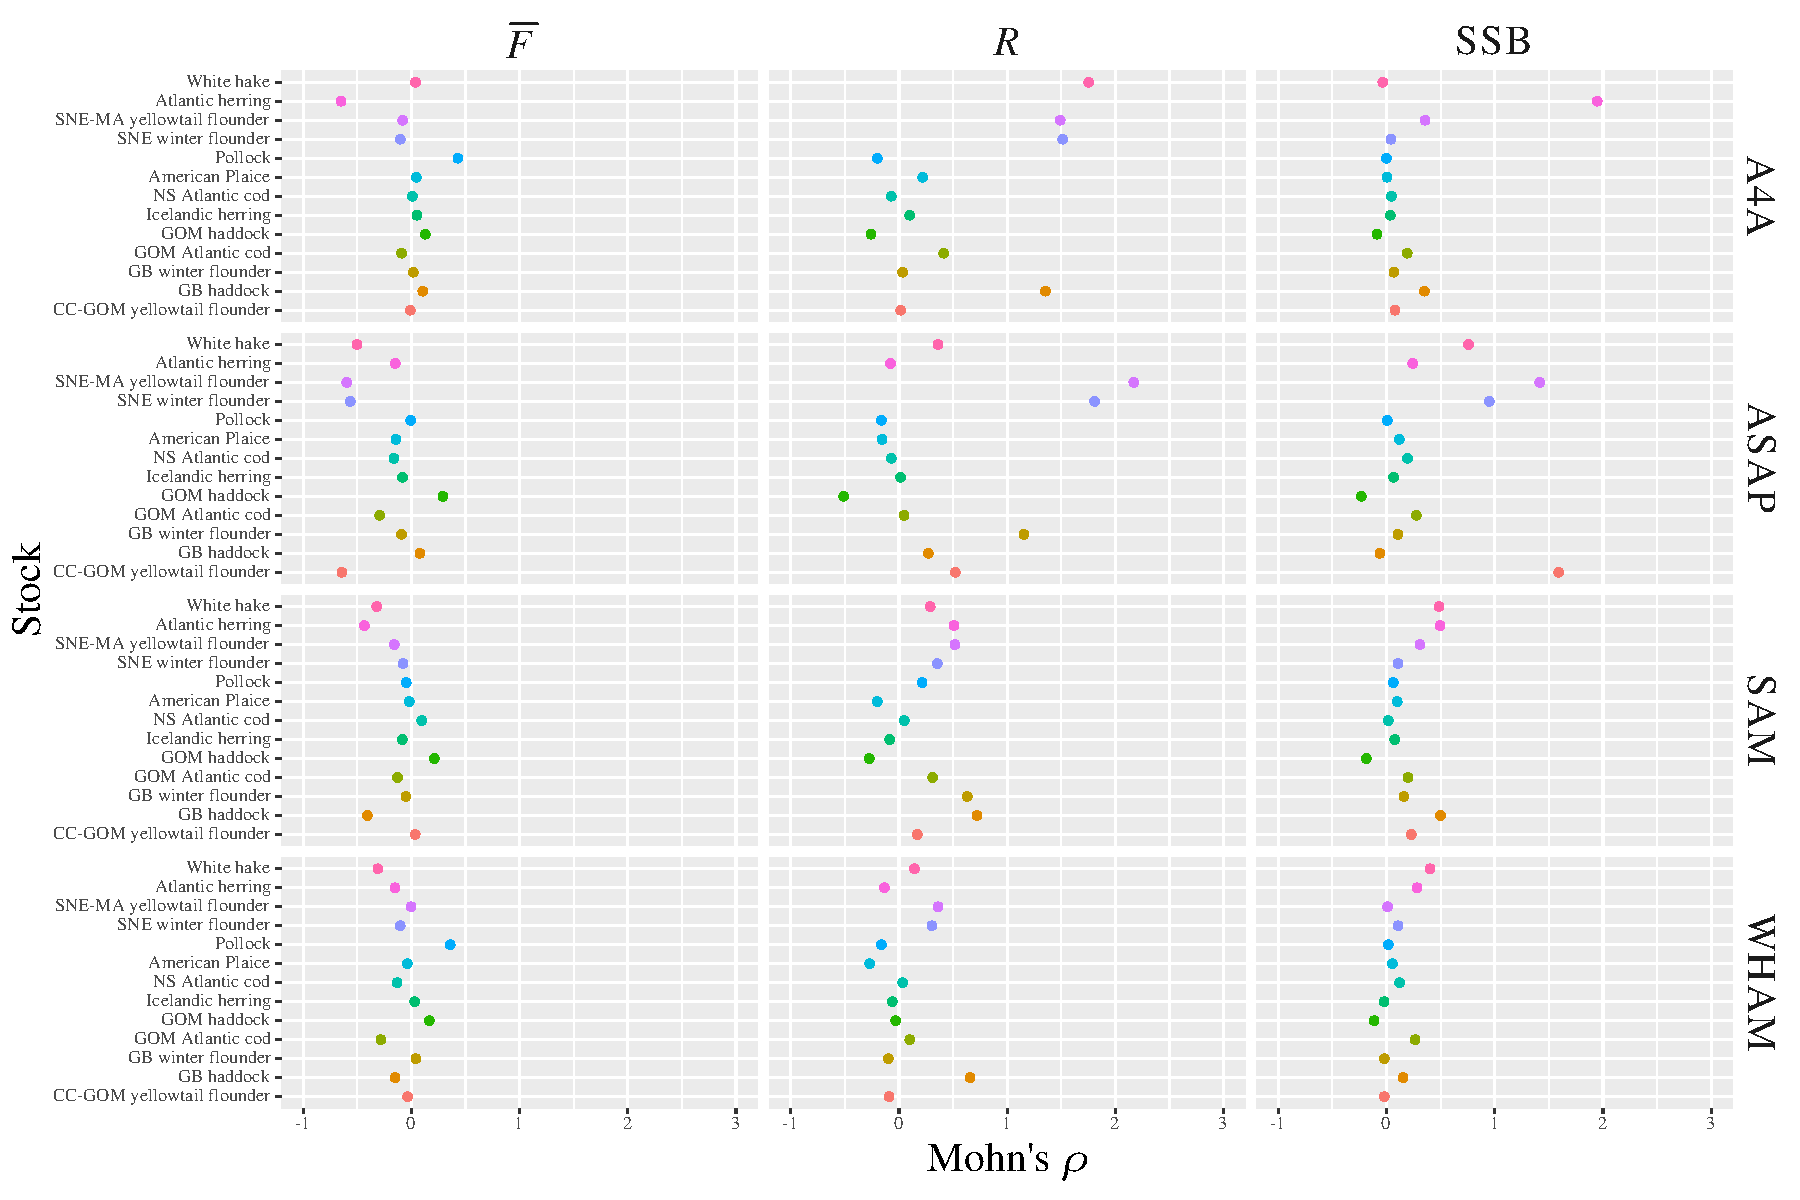
\includegraphics[height = 0.9\textheight]{../db/rho_paper_plot.pdf}
\end{center}
\end{figure}

\begin{figure}
\caption{Relationship between Mohn's $\rho$ for SSB and average fishing mortality by model.}\label{rho_ssb_vs_F}
\begin{center}
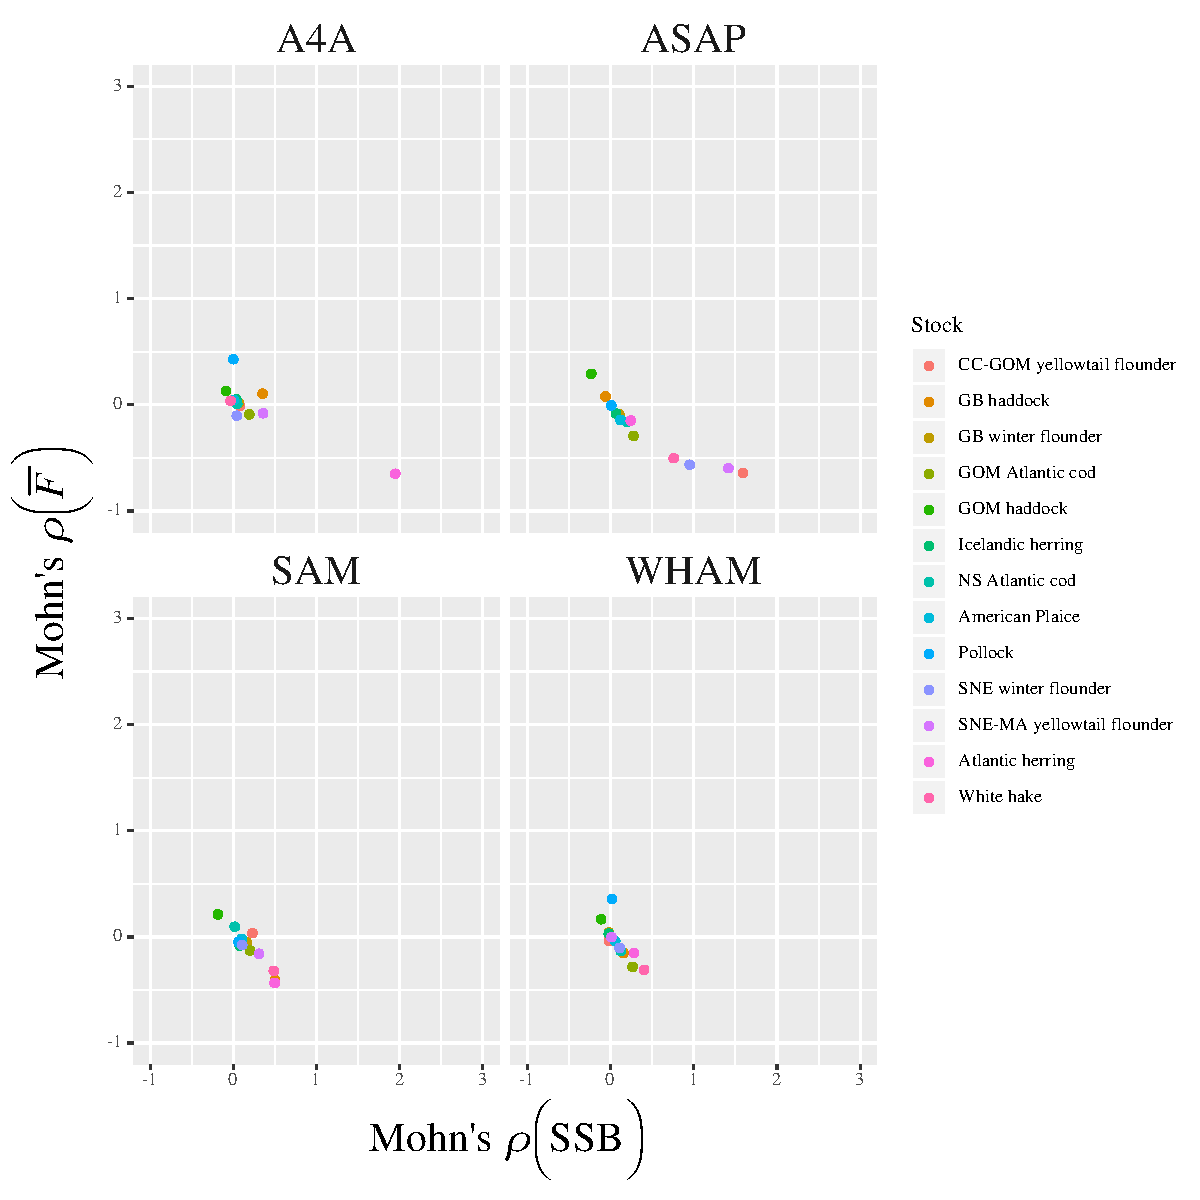
\includegraphics[height = 0.9\textheight]{../db/SSBvsFbarMohnRho_paper.pdf}
\end{center}
\end{figure}

\begin{figure}
\caption{Degree of retrospective pattern in average fishing mortality, recruitment, and spawning stock biomass as measured by Mohn's $\rho$ for each stock and WHAM model configuration.}\label{wham_rho_paper_plot}
\begin{center}
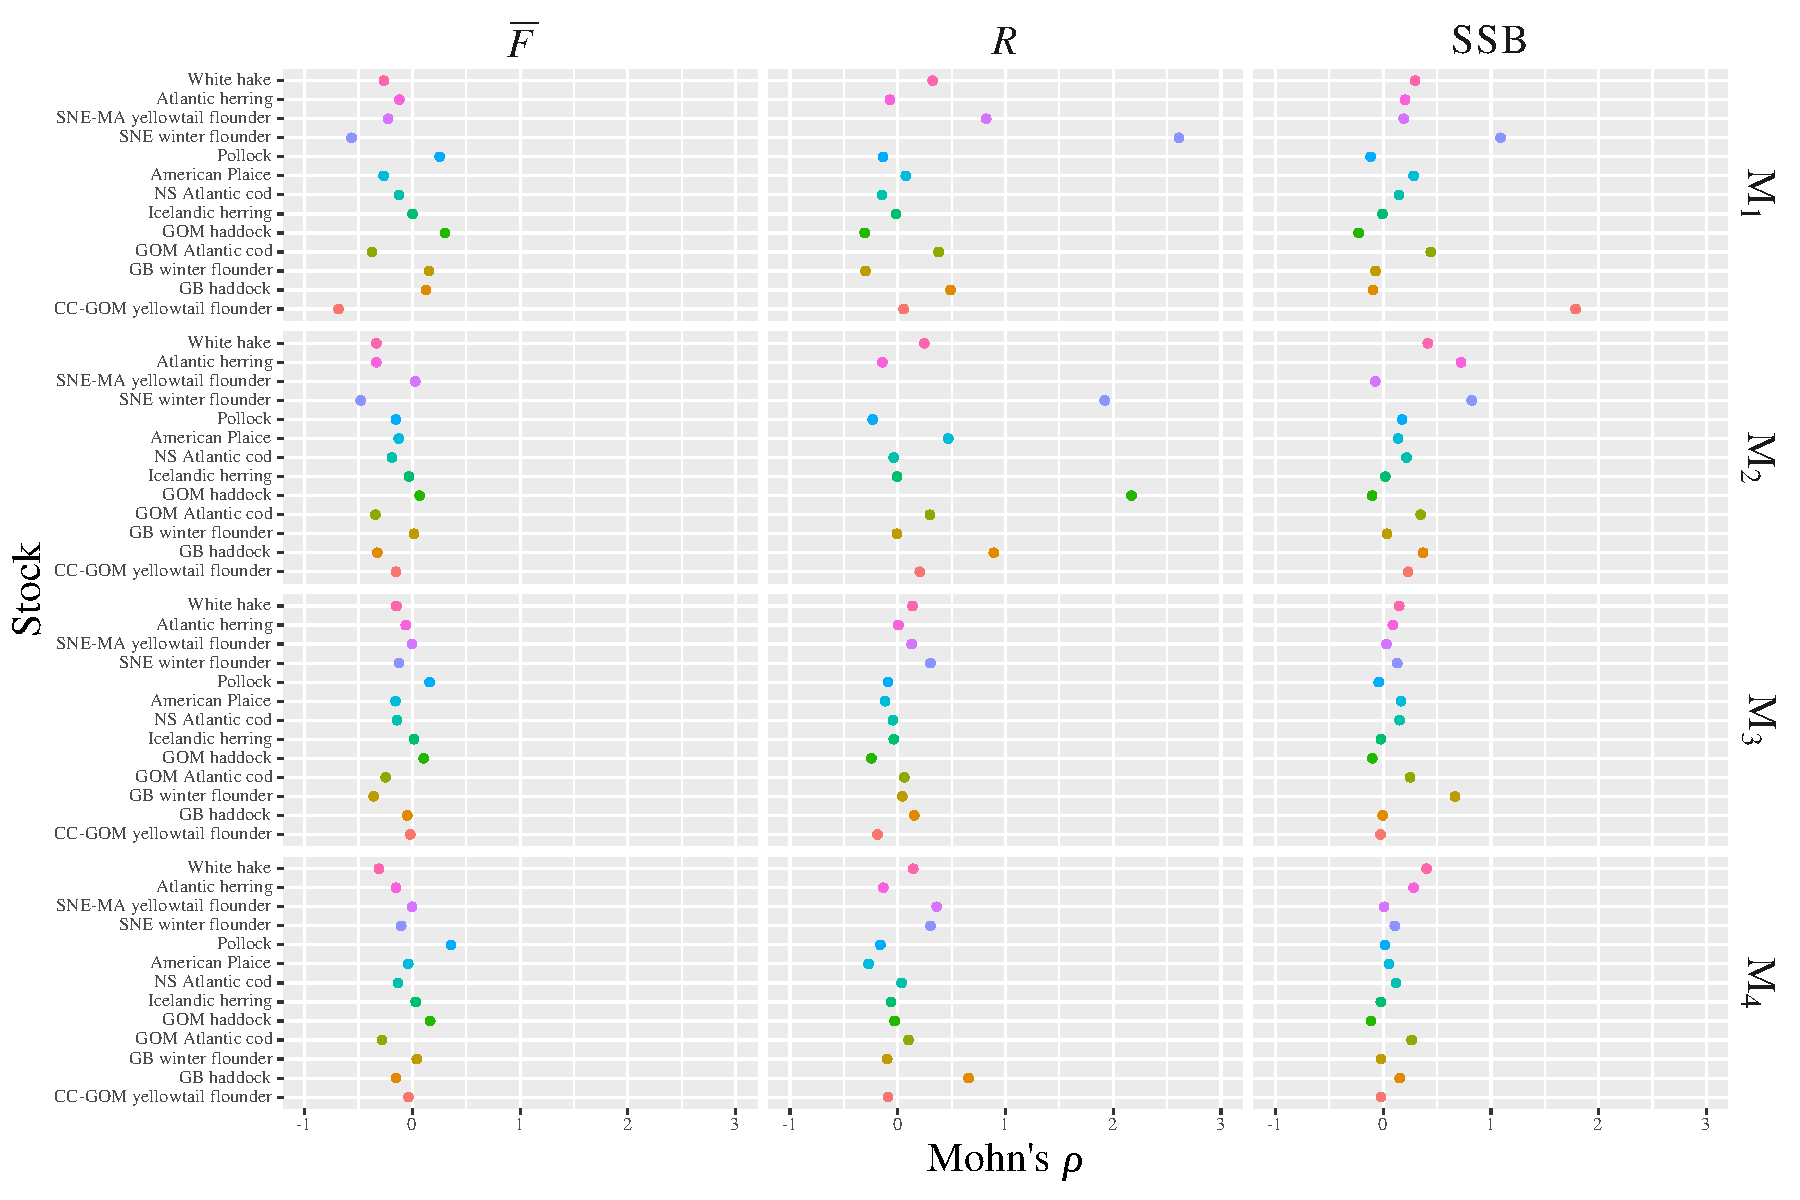
\includegraphics[height = 0.9\textheight]{../db/wham_rho_paper_plot.pdf}
\end{center}
\end{figure}
\end{landscape}

\clearpage

%Tables

\begin{table}
\begin{center}
\caption{Modelling assumptions for the four estimation models.}\label{assumption_models}

\begin{tabular}{lllll}
\toprule
Assumptions & A4A & ASAP & WHAM & SAM\\
\midrule
Fit to total catch & & & LN & \\
Fit to catch age composition & & & Logistic-normal & \\
Fit to catch at age matrix & & & & \\
Fit to total survey index & & & Log-normal & \\
Fit to survey index age composition & & & Logistic-normal & \\
Fit to survey index at age matrix & & & & \\
Recruitment & & & Log-normal random effect& \\
Fishing mortality & & & Fixed effects & \\
Numbers at age & & & Log-normal random effect & \\
Comments & & & & \\
\bottomrule
\end{tabular}

\end{center}
\end{table}

\begin{table}
\begin{center}
\caption{Fish stocks considered in this study.}\label{fish_stocks}
% Possibility of reducing name code and use the same in figures so legend/labels less long
\begin{tabular}{lllll}
\toprule
Fish stock & Name code & Current Model & No. Surveys & Reference\\
\midrule
Cape Cod-Gulf of Maine yellowtail flounder & CC-GOM yellowtail flounder & VPA & 4 & \citet{nefsc17} \\
Georges Bank haddock & GB haddock & VPA & 3 & \citet{nefsc17} \\
Georges Bank winter flounder & GB winter flounder & VPA & 3 & \citet{nefsc17} \\
Gulf of Maine Atlantic cod & GOM Atlantic cod & ASAP & 3 & \citet{nefsc17} \\
Gulf of Maine haddock & GOM haddock & ASAP & 2 & \citet{nefsc17} \\
Icelandic herring & Icelandic herring & VPA & 1 & \\
North Sea Atlantic cod & NS cod & SAM & 2 & \citet{ices18}\\
American plaice & American plaice & VPA & 4 & \citet{nefsc17} \\
Pollock & Pollock & ASAP & 2 & \citet{nefsc17} \\
Southern New England-Mid Atlantic winter flounder & SNE winter flounder & ASAP & 3 & \citet{nefsc17} \\
Southern New England-Mid Atlantic yellowtail flounder & SNE-MA yellowtail flounder & ASAP & 2 & \citet{nefsc17} \\
US Atlantic herring & Atlantic herring & ASAP & 2 & \citet{deroba15} \\
White hake & White hake & ASAP & 2 & \citet{nefsc17} \\
\bottomrule
\end{tabular}

\end{center}
\end{table}

\begin{table}
\begin{center}
\caption{Mean and Standard Deviation of Mohn's $\rho$ for SSB, $\overline{F}$, and recruitment across all stocks by model type.}\label{model_compare}
%latex.default(x[-1], file = "../tex/rho_model_summary.tex", n.rgroup = c(4,     4, 4), rgroup = unique(x$Metric), table.env = FALSE, rowname = NULL,     booktabs = TRUE)%
\begin{center}
\begin{tabular}{lrr}
\toprule
\multicolumn{1}{c}{Model}&\multicolumn{1}{c}{Mean}&\multicolumn{1}{c}{SD}\tabularnewline
\midrule
&&\tabularnewline
A4A&$-0.01$&$0.24$\tabularnewline
ASAP&$-0.22$&$0.28$\tabularnewline
SAM&$-0.11$&$0.19$\tabularnewline
WHAM&$-0.05$&$0.18$\tabularnewline
\midrule
&&\tabularnewline
A4A&$ 1.13$&$2.30$\tabularnewline
ASAP&$ 0.41$&$0.81$\tabularnewline
SAM&$ 0.25$&$0.31$\tabularnewline
WHAM&$ 0.06$&$0.26$\tabularnewline
\midrule
&&\tabularnewline
A4A&$ 0.23$&$0.53$\tabularnewline
ASAP&$ 0.42$&$0.58$\tabularnewline
SAM&$ 0.20$&$0.21$\tabularnewline
WHAM&$ 0.09$&$0.15$\tabularnewline
\bottomrule
\end{tabular}\end{center}

\end{center}
\end{table}

\end{document}
